\chapter{ANALIZA ZAGADNIENIA}

\section{Fizyczne zasady działania akcelerometru i żyroskopu}

\subsection{Akcelerometr}

Zadaniem tego podzespołu jest pomiar i analiza przyspieszenia liniowego/kątowego. Wewnątrz urządzenia znajduje się czujnik przyspieszenia, który bada siłę wynikającą ze zmian ruchu. Dzięki dużej wrażliwości na zmianę położenia jest on w stanie określać z dużą precyzją i dokładnością ruch własny, jak i całego akcelerometru. Najczęściej wykorzystuje się 3-osiowe podzespoły (wykonujące pomiar względem osi OX, OY i OZ). Możemy podzielić je na:

\begin{itemize}
    \item piezoelektryczne - mają duże pasmo pomiarowe. Mogą mierzyć drgania o wysokich częstotliwościach i amplitudach. 
    \item piezorezystancyjne - wykorzystywane do pomiarów wibracji. Stosowane powszechnie w przemyśle.
    \item pojemnościowe MEMS - najmniejsze i najtańsze. Zostały zastosowane w opracowywanym prototypie.
\end{itemize}

W przypadku akcelerometrów MEMS pomiar polega na badaniu zmian pojemności pomiędzy ruchomą masą a nieruchomymi okładkami kondensatora. Podczas ruchu z przyspieszeniem zmienia się pojemność, którą następnie można przekonwertować na potrzebną wartość. Wadą tych elementów (korygowaną stopniowo przez producenta) jest stosunkowo mała czułość i podatność na szumy. Rysunek 3.1 przedstawia przykładową charakterystykę niezamocowanego modułu wprawionego w ruch symulujący ten z tomografu.

\begin{figure}[H]
    \centering
    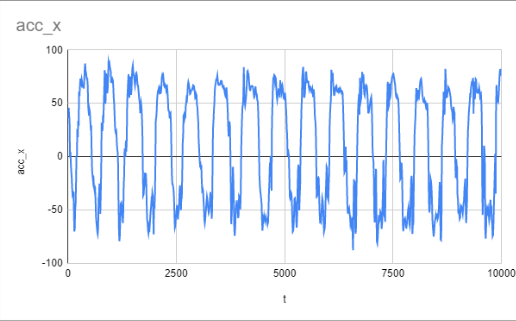
\includegraphics[width=0.9\textwidth]{pictures/raw.png}
    \caption{Przykładowa charakterystyka z akcelerometru A [ref] = f(t [ms])}
    \label{fig:raw}
\end{figure}

\newpage

Dla wartości względem osi OX i OY przesyłanych przez urządzenie stosuje się przekształcenia, umożliwiające otrzymanie odpowiednio: kąta pochylenia (ang. pitch) $\theta$, jak i przechylania (ang. roll) $\phi$ :

\begin{equation}
    \theta = \arctan \Bigg( \frac{A_{x}}{\sqrt{A_{y}^{2} + A_{z}^{2}}} \Bigg)
\end{equation}
\begin{equation}
    \phi = \arctan \Bigg( \frac{A_{y}}{\sqrt{A_{x}^{2} + A_{z}^{2}}} \Bigg)
\end{equation}

Powyższe wzory wynikają bezpośrednio z twierdzenia Pitagorasa zastosowanego w przestrzeni trójwymiarowej ($A$ - wektor przyspieszenia).

\subsection{Żyroskop}

Żyroskopy to urządzenia służące do analizy, jak i utrzymywania orientacji przestrzennej. Można je podzielić na kierunkowe, prędkościowe i elektroniczne. Służą do mierzenia prędkości obrotowej obiektu. Drgania elementu zostają wymuszone dzięki efektowi piezoelektrycznemu, natomiast pomiar wykorzystuje siłę Coriolisa (złożenie dwóch ruchów pewnej masy, z czego jeden jest ruchem  obrotowym) \cite{filtr}.

By otrzymać zmianę kąta, otrzymane dane należy scałkować po czasie, co prezentują poniższe równania \cite{filtr}:

\begin{equation}
    \theta(t_{i}) = \theta(0) + \sum^{i}_{j=1} \omega_{X}(t_{j})(t_{j} - t_{j-1})
\end{equation}
\begin{equation}
    \phi(t_{i}) = \phi(0) + \sum^{i}_{j=1} \omega_{Y}(t_{j})(t_{j} - t_{j-1}),
\end{equation}
\begin{equation}
    \psi(t_{i}) = \psi(0) + \sum^{i}_{j=1} \omega_{Z}(t_{j})(t_{j} - t_{j-1}),
\end{equation}

\noindent gdzie: $\theta$ - kąt przechylania (pitch), $\phi$ - kąt pochylania (roll), $\psi$ - kąt skręcenia (yaw), $\omega$ - prędkość obrotowa i jej odpowiednie składowe względem danej osi, $t$ - czas.

\subsection{Filtr Kalmana}

Otrzymywane pomiary podatne są na zakłócenia: akcelerometr jest wyczulony na drgania otoczenia, natomiast żyroskop jest podatny na zjawisko dryfu. Dodatkowo, ze względu na dane z dwóch czujników, należy dokonać ich złożenia. Do tego celu stosuje się między innymi  filtr Kalmana, który dokonuje iteracyjnej estymacji procesu w układzie ze sprzężeniem zwrotnym \cite{filtr}. Możemy wyznaczyć dwie fazy działania filtru: fazę predykcyjną i fazę korekcji.

W praktyce zostanie wykorzystany cyfrowy filtr Kalmana realizujący algorytm rekurencyjny. Bazując na \cite{kal}, model estymacji możemy przedstawić jako: liniowe równanie stanu i liniowe równanie obserwacji (odpowiednio (3.6) i (3.7)).

\newpage

\begin{equation}
    x(t+1) = A(t)x(t) + B(t)v(t)
\end{equation}
\begin{equation}
    y(t) = C(t)x(t) + w(t)
\end{equation}

\noindent gdzie: $t$ - wartości dyskretne na osi czasu, $x(t)$ - wektor stanu, $y(t)$ - wektor obserwacji, $v(t)$ - biały szum procesowy o zerowej wartości średniej, $w(t)$ - biały szum obserwacji o zerowej wartości średniej, $A(t)$ - macierz systemowa, $B(t)$ - macierz wejścia, $C(t)$ - macierz wyjścia.

Następnie w fazie korekcji algorytm wykorzystuje pomiary do aktualizacji i poprawy estymacji. W publikacji \cite{kal} została przedstawiona dalsza metodologia działania tych filtrów.

\section{Płytka Arduino Uno}

Arduino to projekt rozpoczęty w roku 2005, opierający się na licencji typu \textit{open hardware}. Przeznaczony on jest dla mikrokontrolerów zamontowanych na obwodzie drukowanym z wbudowanymi układami wejścia/wyjścia (I/O) oraz standaryzowanym językiem programowania. Ostatni bazuje na C++, a wykorzystując wtyczkę PlatformIO możliwe jest kompletne posługiwanie się tym językiem.

W projekcie zostanie wykorzystany model Arduino Uno. Został on wybrany na podstawie dostępnych funkcjonalności, przy akceptowalnej cenie produktu. Opracowywane oprogramowanie nie będzie zapisywać danych na płytce, lecz będą one przesyłane i przechowywane w aplikacji okienkowej. 

\begin{figure}[H]
    \centering
    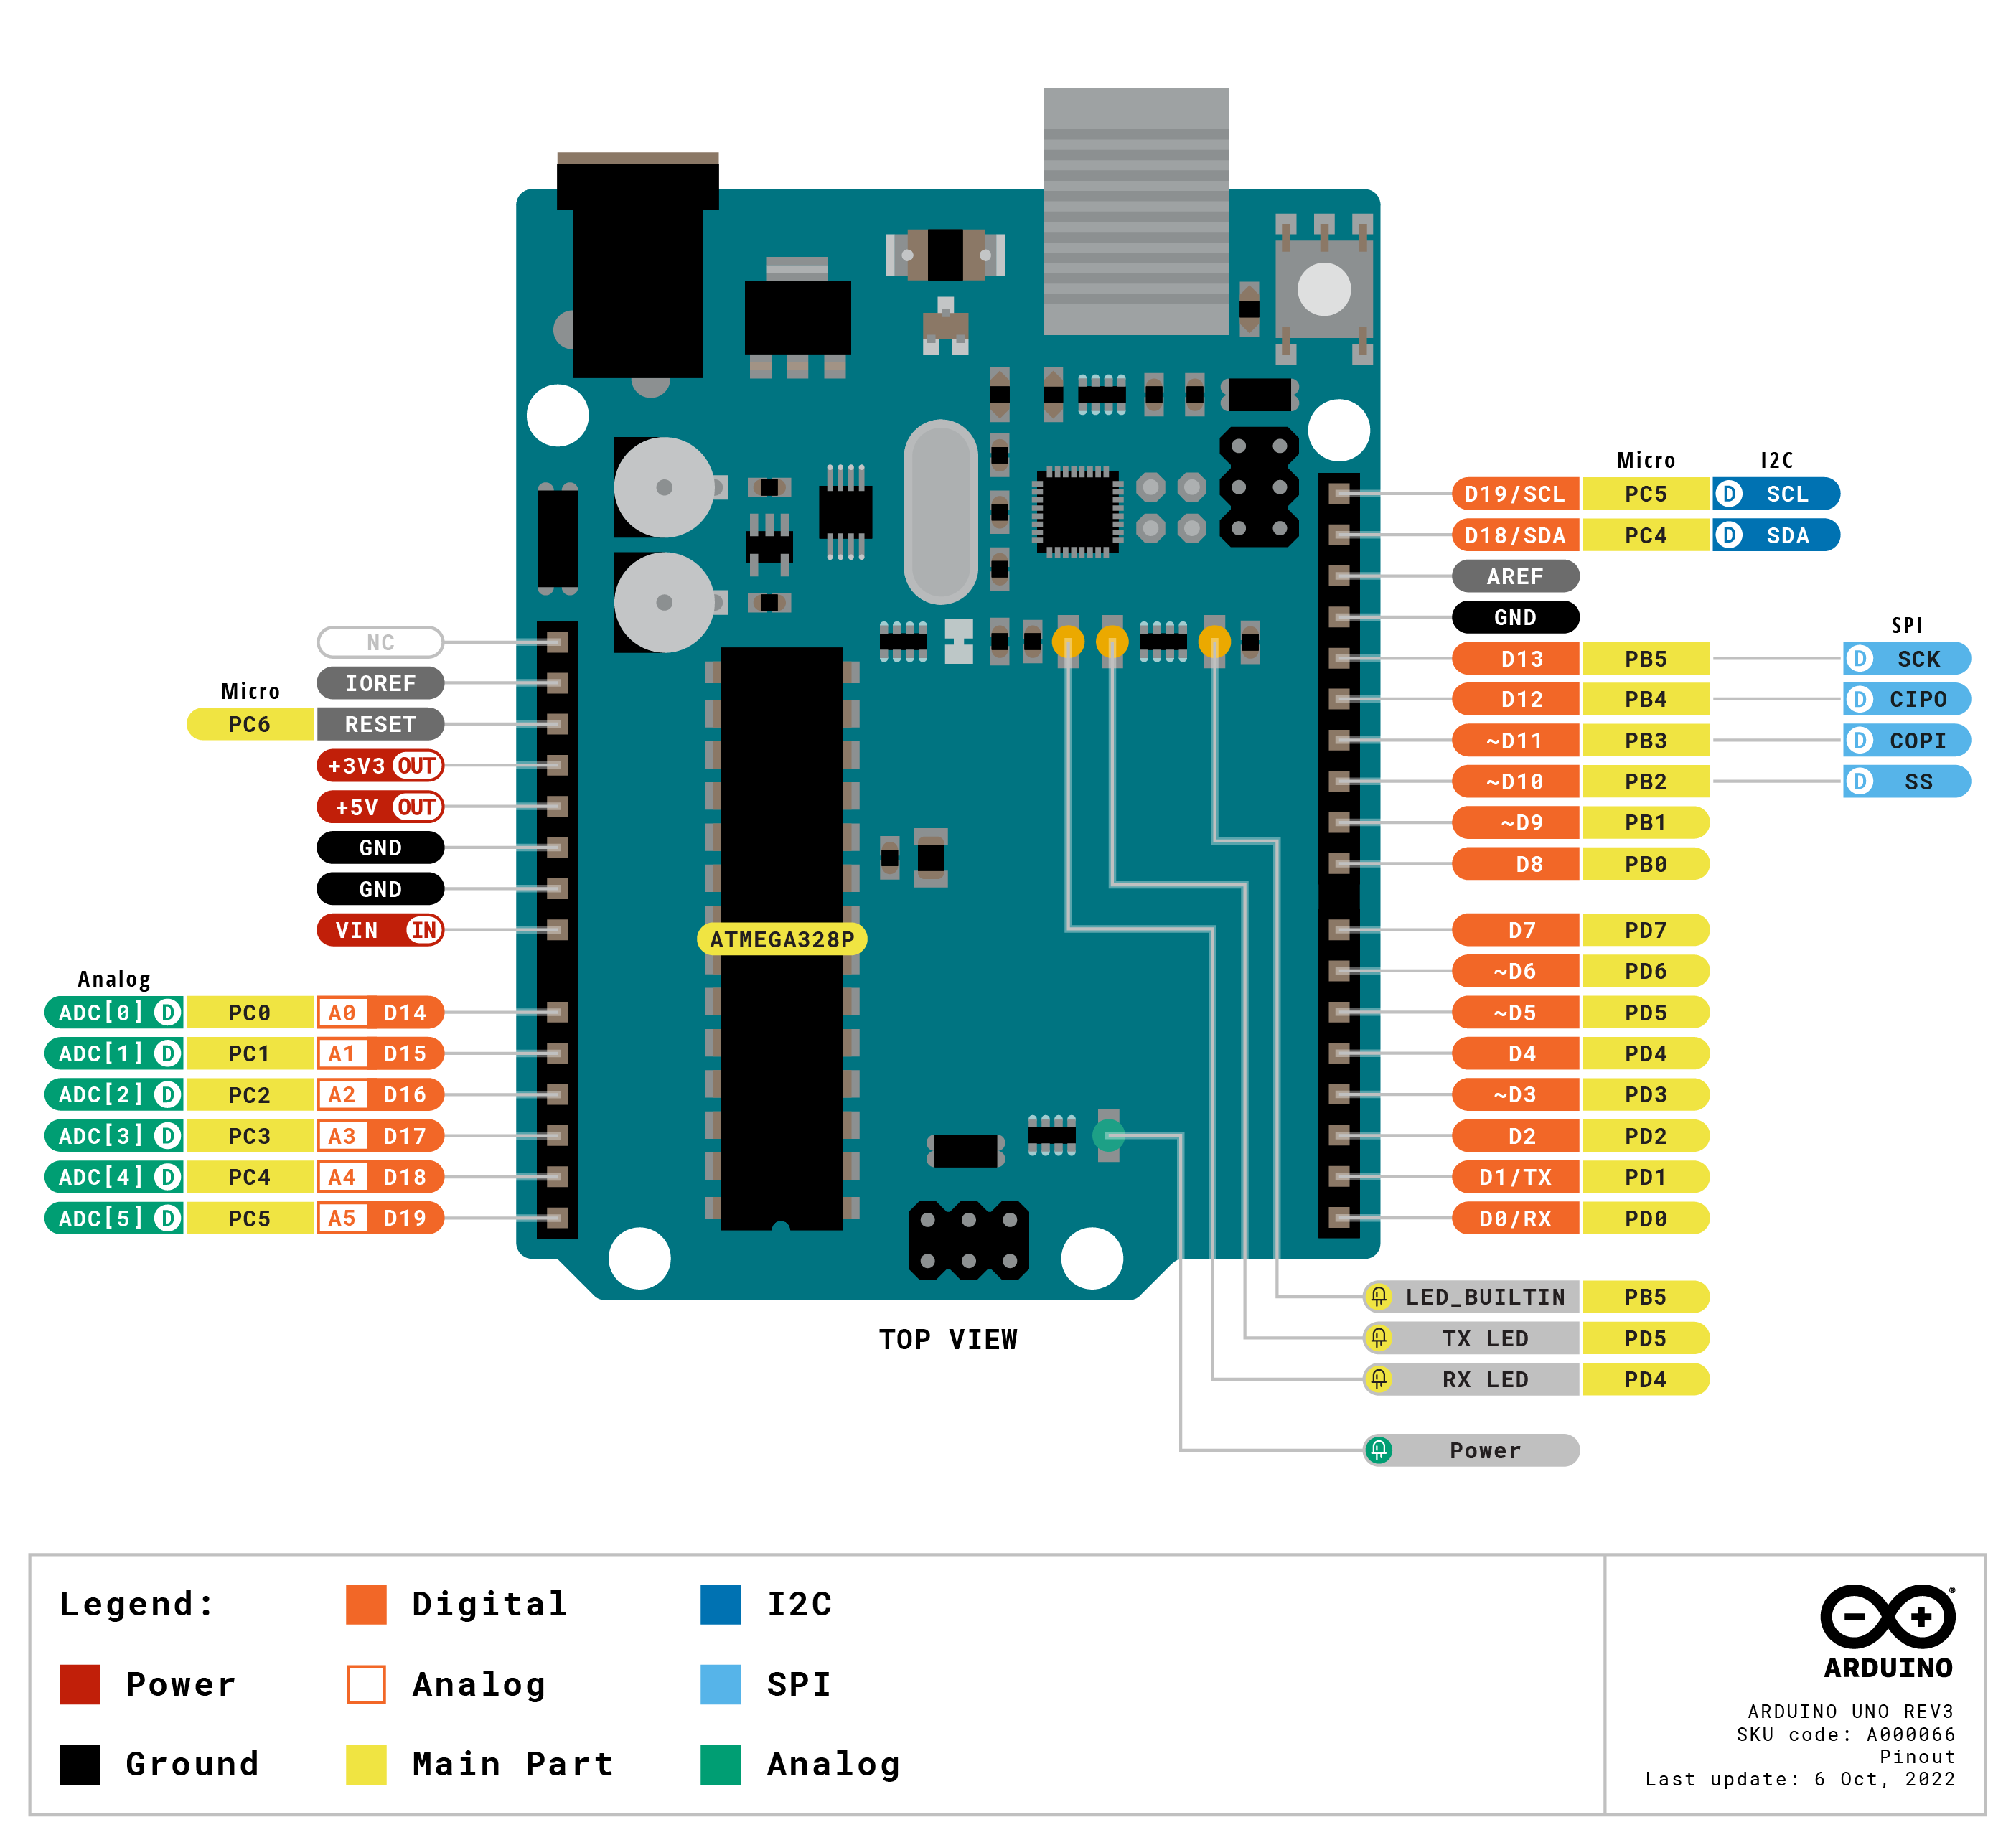
\includegraphics[width=0.9\textwidth]{pictures/uno.png}
    \caption{Schemat Arduino Uno \cite{Ardocs}}
    \label{fig:ard_vague}
\end{figure}

Sama płytka składa się z 8-bitowego mikrokontrolera Atmel AVR (konkretnie ATmega328P), ma wbudowane 32KB pamięci flash, 2KB SRAM, 1KB EEPROM. Posiada interfejsy: I2C, SPI, UART i USB (jest programowana przez adapter \textit{USB to serial}). Działa na napięciach wejścia 7-12V oraz wartościach napięć operacyjnych 3.3V i 5V. Płytka posiada 20 pinów cyfrowych oraz 6 analogowych i typu PWM. Rys. 3.2 przedstawia umiejscowienie powyższych funkcji na płytce drukowanej.

Oficjalnym środowiskiem do programowania omawianych płytek jest Arduino IDE. Aczkolwiek, ze względu na stosunkowo ograniczone możliwości w pracy zostanie wykorzystane JetBrains CLion wraz z wtyczką PlatformIO. Oprogramowanie to posiada znacznie większe możliwości, jako że producent specjalizuje się w narzędziach programistycznych, zarówno na licencjach płatnych, jak i tych typu \textit{open source}.

\section{Moduł DFRobot SEN0142 (MPU-6050) - dodatek do Arduino}

MPU-6050 opracowane przez firmę InvenSense są powszechnie używane w modułach określających położenie w przestrzeni, jak i prędkością obrotową. Charakteryzują się one małym poborem mocy oraz wysoką wydajnością. Podzespoły te zawierają w sobie dwa analogowe czujniki: akcelerometr i żyroskop. Oba pozwalają na pomiar zmiany kąta, jednak na odmiennej zasadzie. Sam moduł posiada wbudowany cyfrowy procesor ruchu, jak i 16-bitowy przetwornik analogowo-cyfrowy (ADC). Wykorzystując magistralę I2C wraz z wbudowanymi rezystorami, możliwe jest (poprzez komunikację szeregową) uzyskanie zestawów danych przy bezpośrednim połączeniu układu z Arduino.

Na rynku jest dostępnych wiele podzespołów z wbudowanym układem MPU-6050. Moduł od firmy DFRobot został wytypowany ze względu na posiadanie funkcji wystarczających do spełnienia założeń doświadczenia przy akceptowalnej cenie. Dodatkowym atutem jest rozmiar czujnika, który całkowicie mieści się na elemencie obrotowym silnika krokowego. Rys. 3.3 prezentuje zespolenie MPU-6050 z całym modułem SEN0142.

\begin{figure}[H]
    \centering
    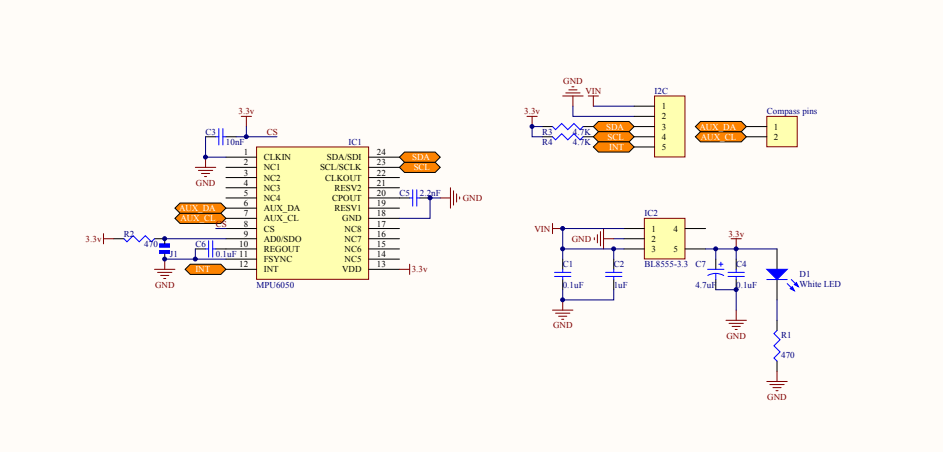
\includegraphics[width=\textwidth]{pictures/short_schema.png}    
    \caption{Schemat modułu DFRobot SEN0142 \cite{shop}}
    \label{fig:DFRobot_scheme}
\end{figure}

\newpage

\subsection*{Specyfikacja na podstawie \cite{dfr}}

\begin{enumerate}
    \item \textbf{Akcelerometr}
    \begin{itemize}
        \item Trzyosiowy, z cyfrowym wyjściem, programowalny w zakresie przeciążeń: $\pm 2\;g$, $\pm 4\;g$, $\pm 8\;g$ i $\pm 16\;g$
        \item Posiada zintegrowane, 16-bitowe przetworniki ADC, pozwalające na próbkowanie sygnałów bez stosowania multiplekserów
        \item Natężenie prądu roboczego: $500 \mu A$
        \item Natężenie prądu przy niskim poborze mocy: $10\; \mu A$ dla $1.25\; Hz$, $20\; \mu A$ dla $5\; Hz$, $60\; \mu A$ dla $20\; Hz$, $110\; \mu A$ dla $40\; Hz$
    \end{itemize}
    \item \textbf{Żyroskop}
    \begin{itemize}
        \item Trzyosiowy, z cyfrowym wyjściem, programowalny w przedziale prędkości kątowych: $\pm 250$, $\pm 500$,  $\pm 1000$ i  $\pm 2000 ^{o}/s$
        \item Wbudowane 16-bitowe ADC
        \item Poprawiona wydajność (względem poprzednich modeli) szumów przy niskich częstotliwościach
        \item Programowalny cyfrowy filtr dolnoprzepustowy
        \item Natężenie prądu roboczego: $3.6\; mA$
        \item Natężenie prądu spoczynkowego: $5\; \mu A$
    \end{itemize}
\end{enumerate}



\section{Budowa i założenia działania czujnika}

\subsection{Budowa}

Czujnik składa się z dwóch elementów: płytki Arduino oraz modułu DFRobot SEN0142 połączonych czterema przewodami, jak pokazano na Rys. 3.4.

\begin{figure}[H]
    \centering
    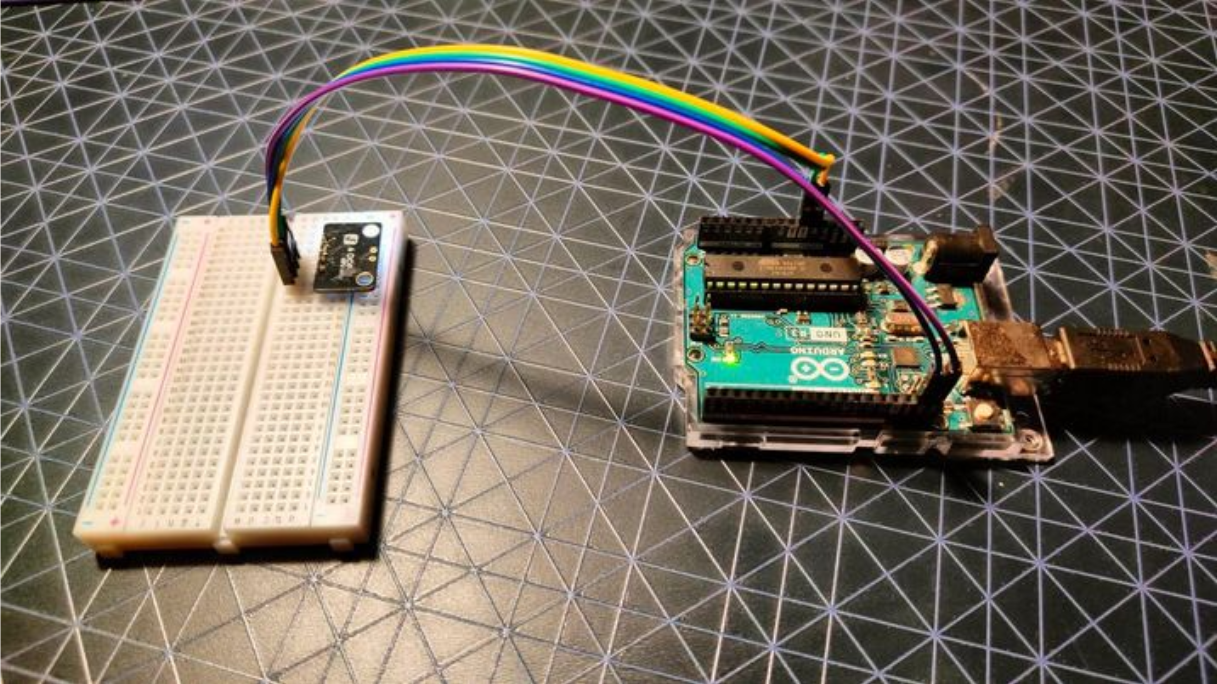
\includegraphics[width=\textwidth]{pictures/prototype.png}
    \caption{Pierwszy prototyp urządzenia}
    \label{sketch}
\end{figure}

Moduł SEN0142 zasilany jest stałym napięciem 5V. SDA i SCL są pinami magistrali I2C odpowiadającymi odpowiednio za: linię danych (serial data) oraz linię zegara taktującego tranmisję (serial clock).

\subsection{Magistrala I2C i port szeregowy}
Komunikacja pomiędzy Arduino a modułem SEN0142 przebiega poprzez szynę I2C. Jak przedstawiono w \cite{forbot}, obie linie magistrali są dwukierunkowe, rezystor podciągający podłącza je do dodatniego napięcia. Gdy nie ma transmisji, to zarówno na SDA i SCL znajduje się stan wysoki. Standardowo dane są przesyłane z prędkością 100 kb/s, lub 400 kb/s. 

Każdy układ podłączony do magistrali ma przypisany adres i może być zarówno odbiornikiem jak i nadajnikiem. Dzielimy je na tzw.: master i slave. Pierwszy inicjuje transmisję i generuje sygnał zegarowy. Drugim natomiast jest każdy zaadresowany układ. Rola mistrza najczęściej jest przypisana mikrokontrolerom, podobnie w przypadku tego projektu: płytce Arduino. 

Napięcia poziomów logicznych nie są zdefiniowane, ale zależą od napięcia zasilającego $V_{dd}$. Jeden impuls zegarowy przypada na każdy przesłany bit. Dla wysokiego poziomu zegara wymagana jest stabilność danych na lilii SDA. Stan może się zmieniać dla niskiego zegara.

\begin{figure}[H]
    \centering
    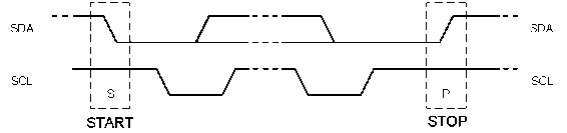
\includegraphics[width=0.95\textwidth]{pictures/ss.png}
    \caption{Bity start i stop \cite{forbot}}
    \label{fig:ss}
\end{figure}

Gdy na SCL panuje stan $1$ a na SDA następuje zmiana:

\begin{itemize}
    \item $1 \rightarrow 0$, następuje bit START,
    \item $0 \rightarrow 1$, następuje bit STOP.
\end{itemize}

Obie sytuacje są generowane przez układ master. Po bicie START szyna jest zajęta, a po STOP się zwalnia.

Komunikacja pomiędzy Arduino a komputerem stacjonarnym odbywa się poprzez UART, kabel USB i port szeregowy.

\begin{figure}[H]
    \centering
    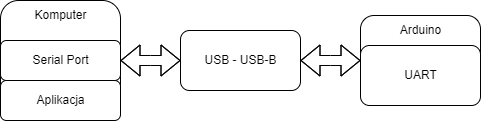
\includegraphics[width=0.8\textwidth]{pictures/serialPort.png}
    \caption{Schemat komunikacji}
    \label{fig:sp}
\end{figure}

Port szeregowy jest typem portu komputerowego, gdzie przekazane dane mają formę ciągu bitów. Jest zdolny do tłumaczenia bitów na bajty i odwrotnie. Jako, że komputer posiada kilka takich portów, należy upewnić się, który z nich przypada na Arduino. Otwierając komunikację istnieje również opcja między innymi: wyboru prędkości połączenia.